\section{Конструкторский раздел}

\subsection{Диаграмма вариантов использования}

\subsection{Диаграмма классов}
На рисунках \ref{fig:dataLayer} -- \ref{fig:serverAndProtocol} предоставлены диаграммы классов компонентов приложения.

\begin{figure}[H]
\begin{center}
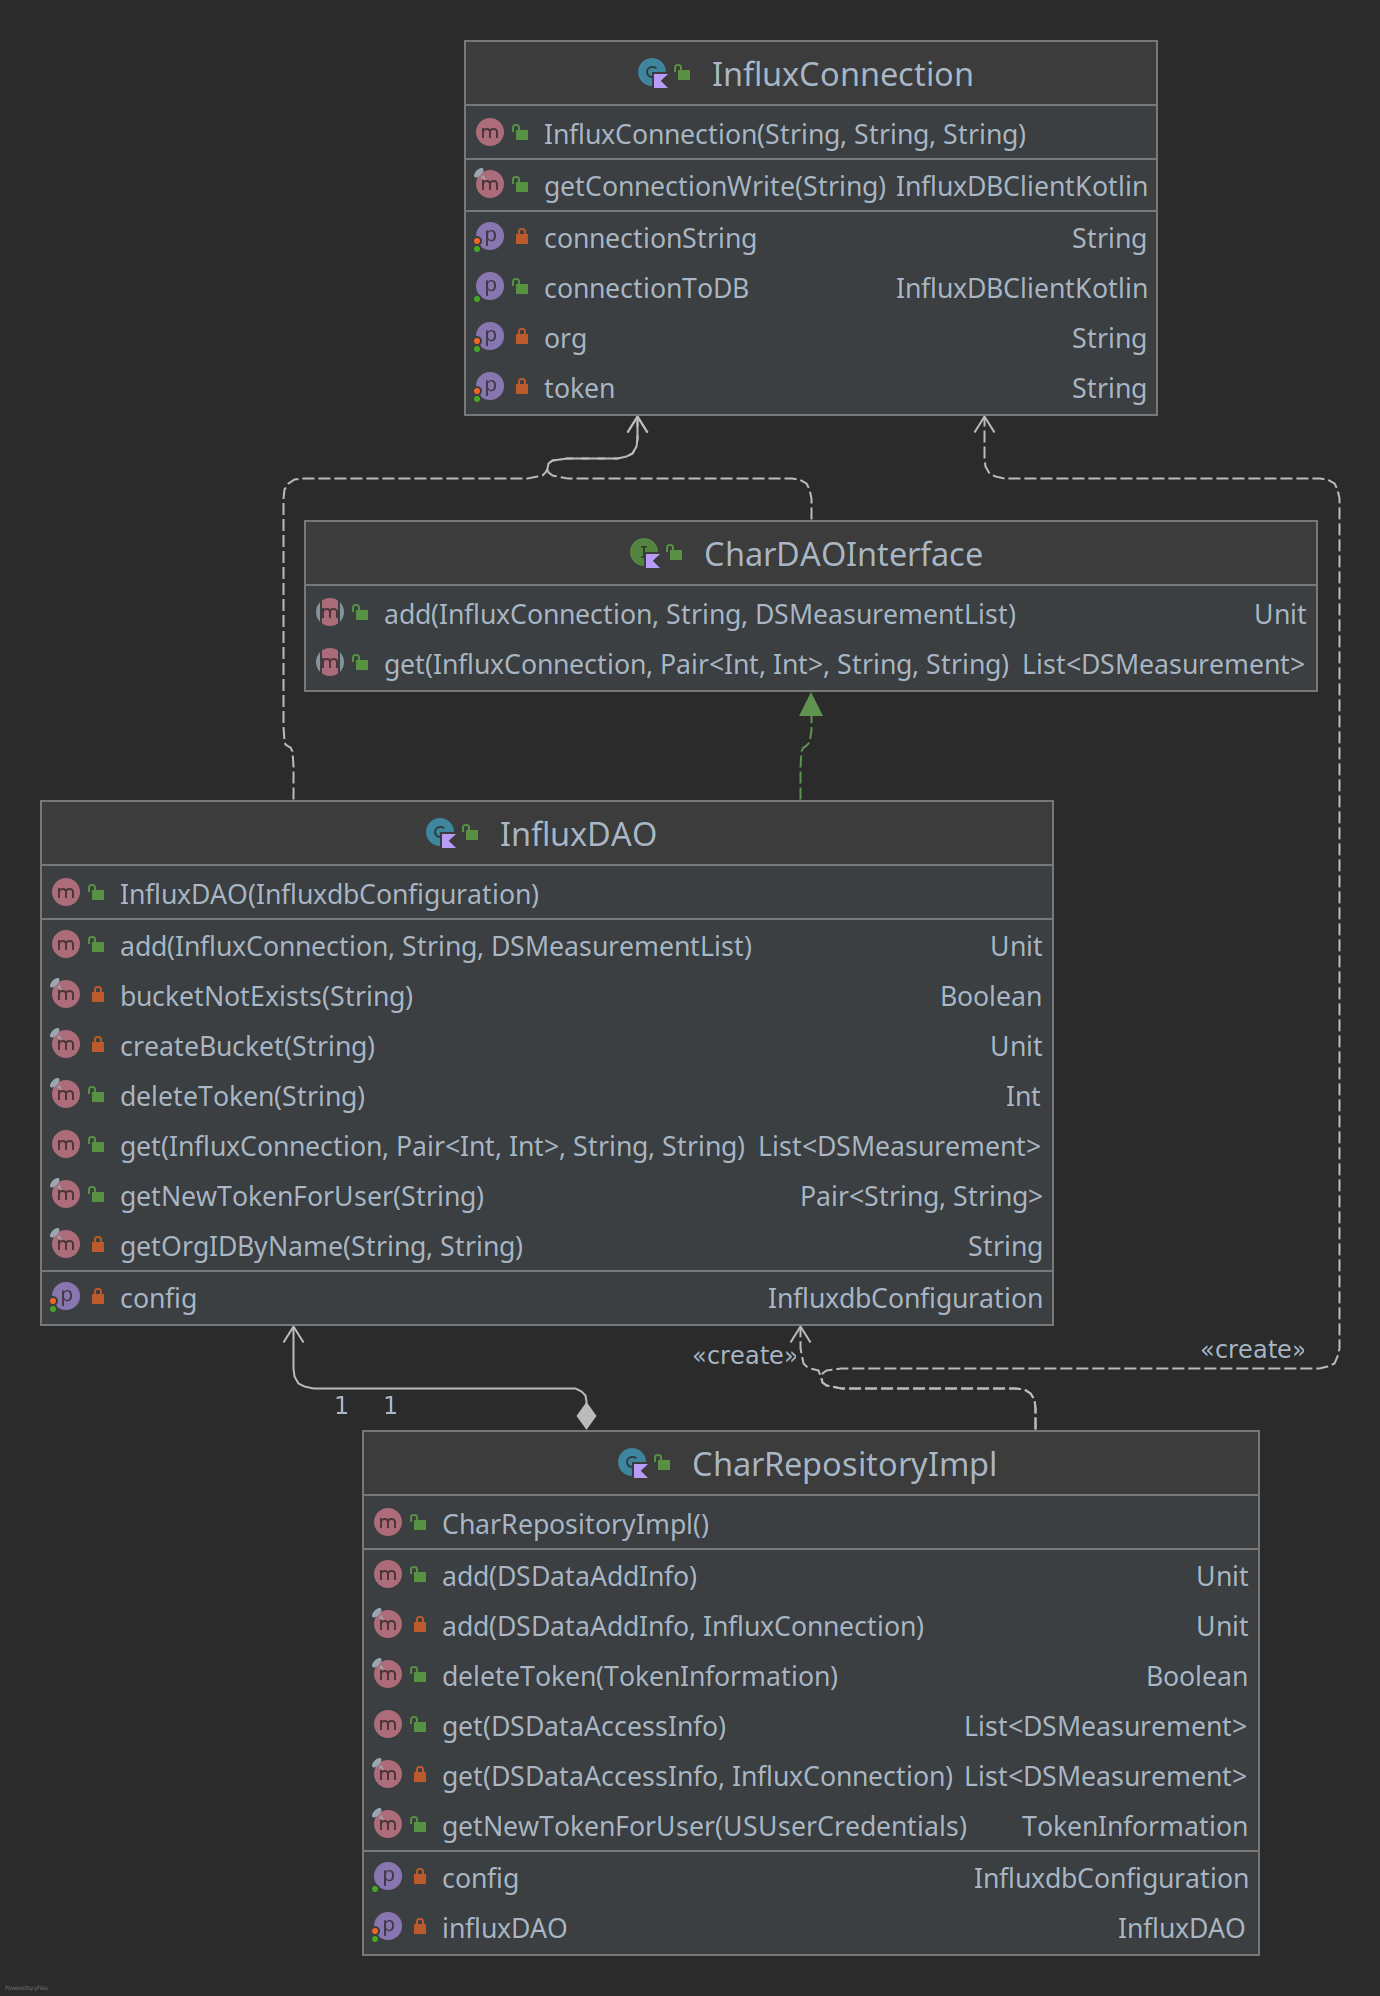
\includegraphics[width=\textwidth]{img/dataLayerDiagram.png}
\captionsetup{justification=centering}
	\caption{Диаграмма классов слоя доступа к данным приложения. }
	\label{fig:dataLayer}
\end{center}
\end{figure}

\begin{figure}[hbtp]
	\centering
	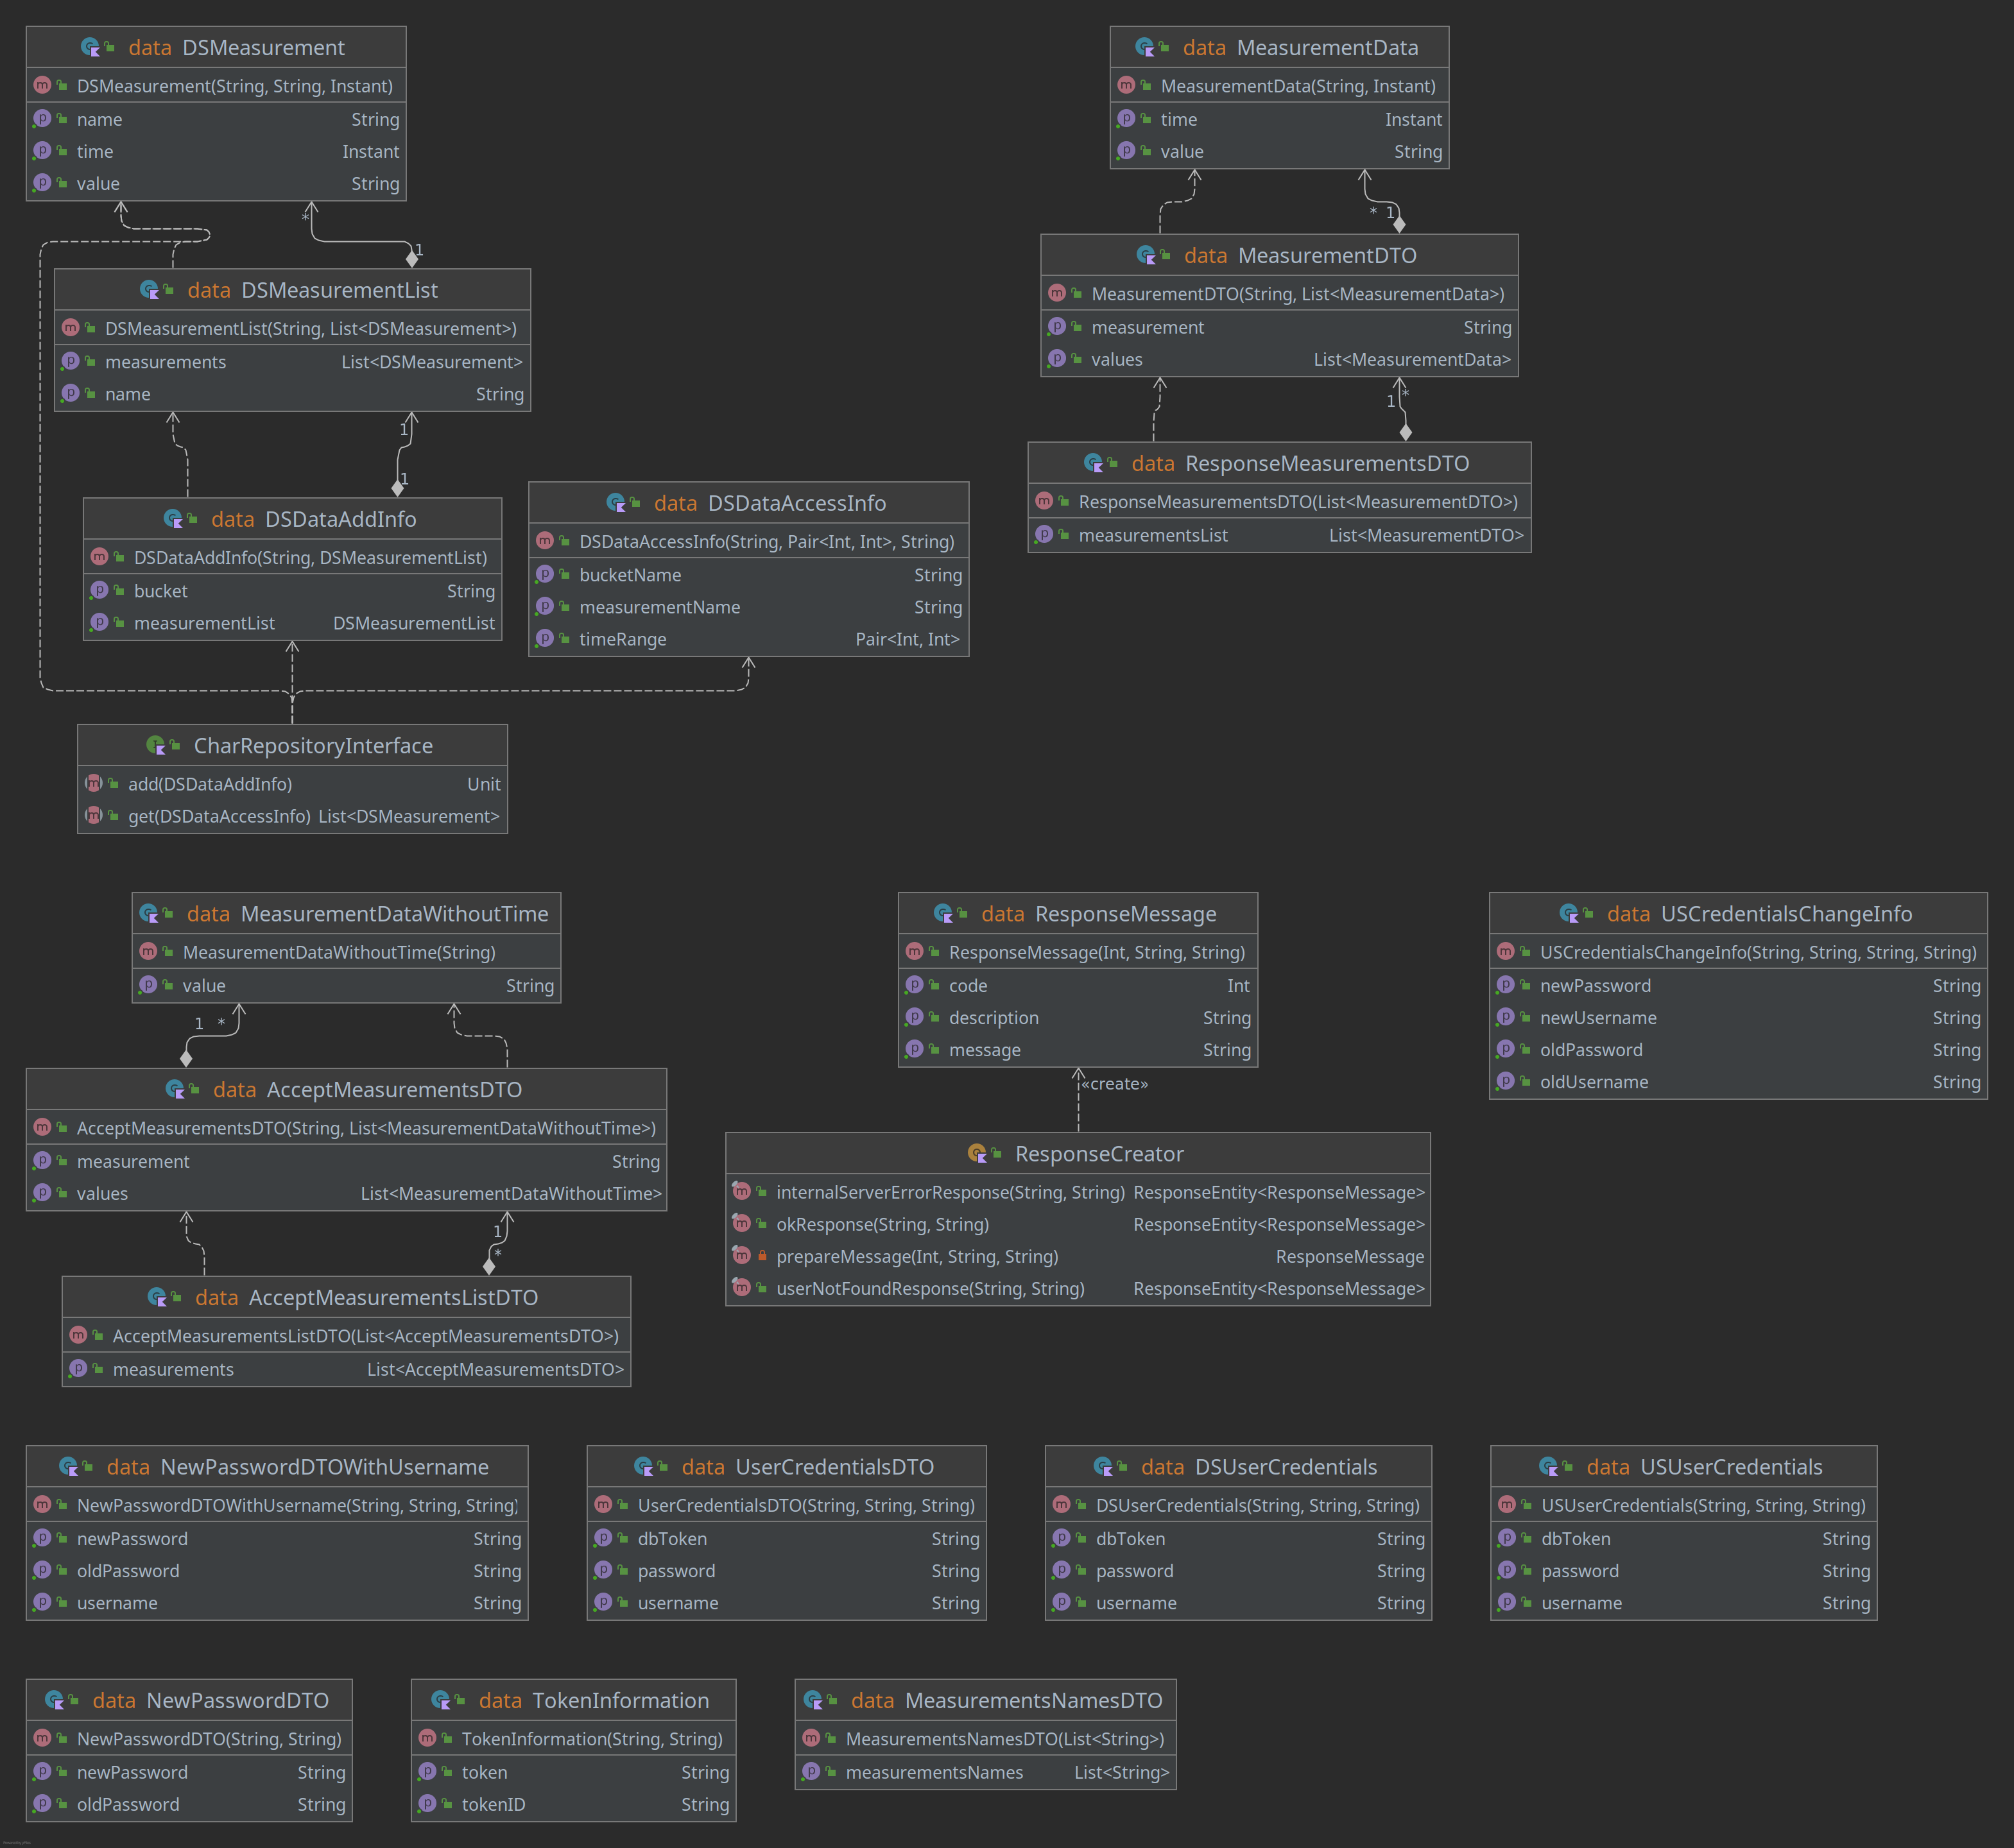
\includegraphics[width=\textwidth]{img/domainLayerDiagram.png}
	\caption{Диаграмма классов бизнес-логики приложения}
	\label{fig:domainLayer}
\end{figure}

\begin{figure}[hbtp]
	\centering
	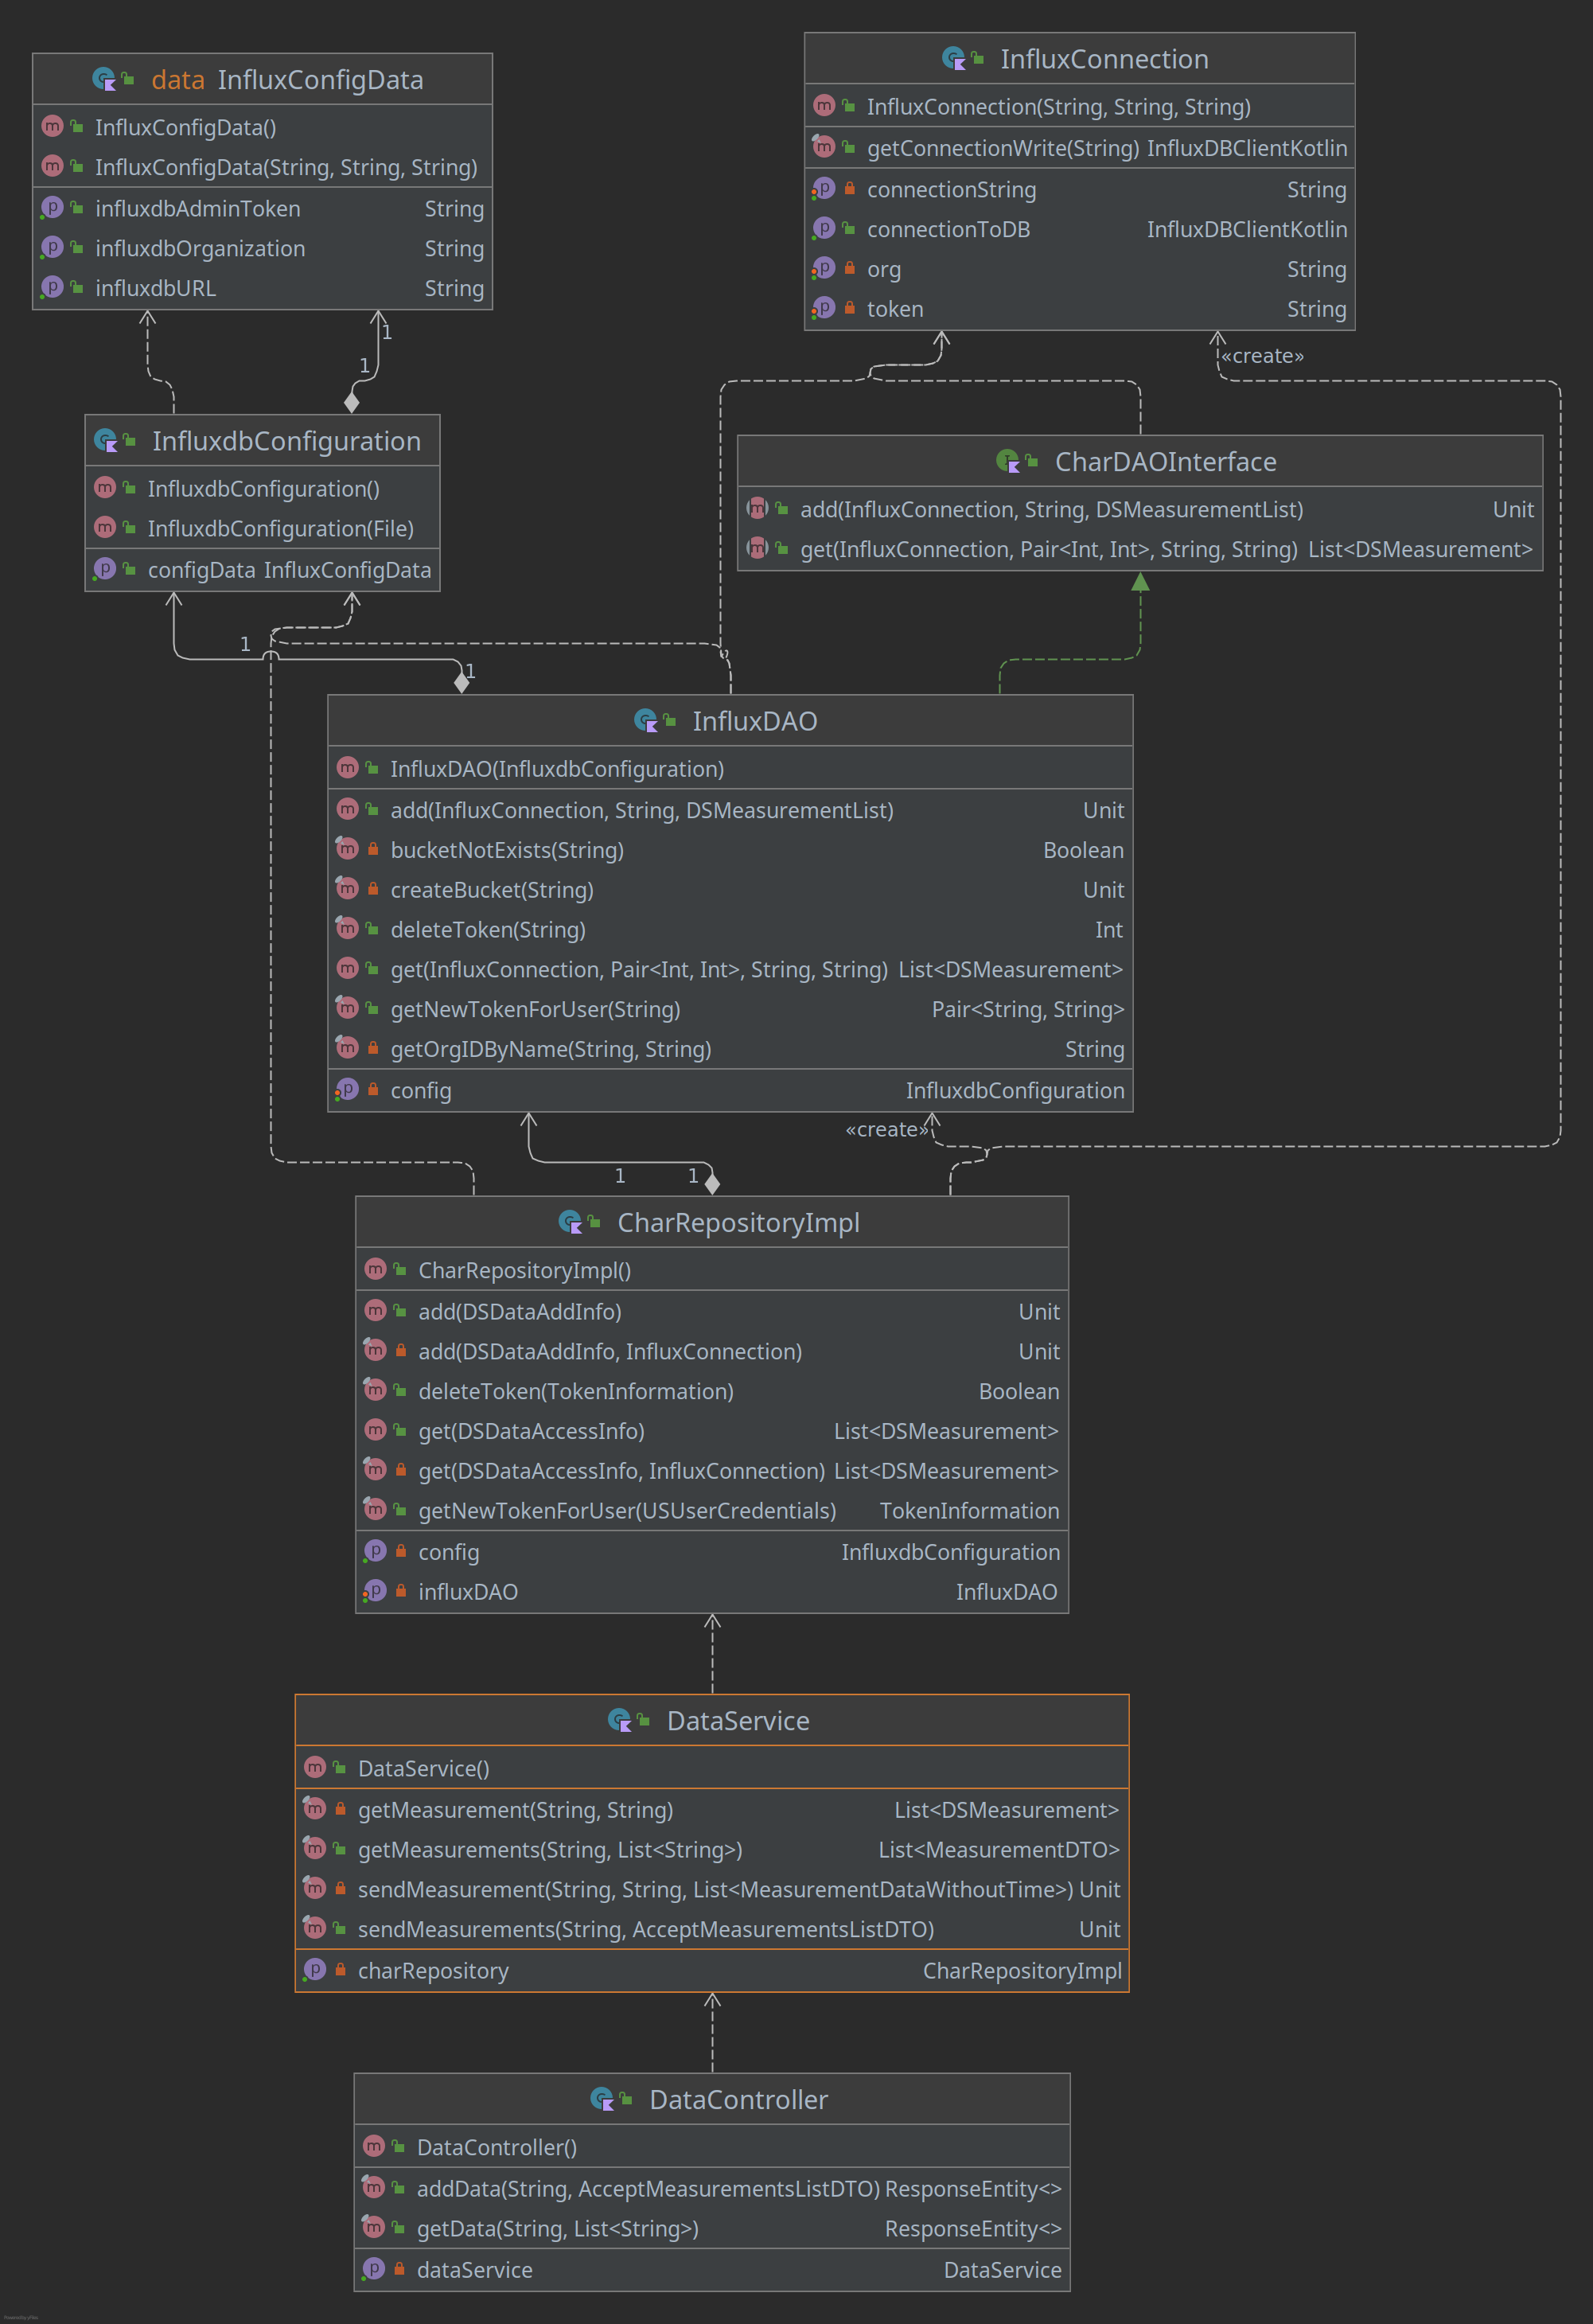
\includegraphics[width=\textwidth]{img/dataAndControllerLinkageDiagram.png}
	\caption{Диаграмма классов, показывающая связь контроллера и слоя доступа к данным}
	\label{fig:dataAndController}
\end{figure}

\begin{figure}[hbtp]
	\centering
	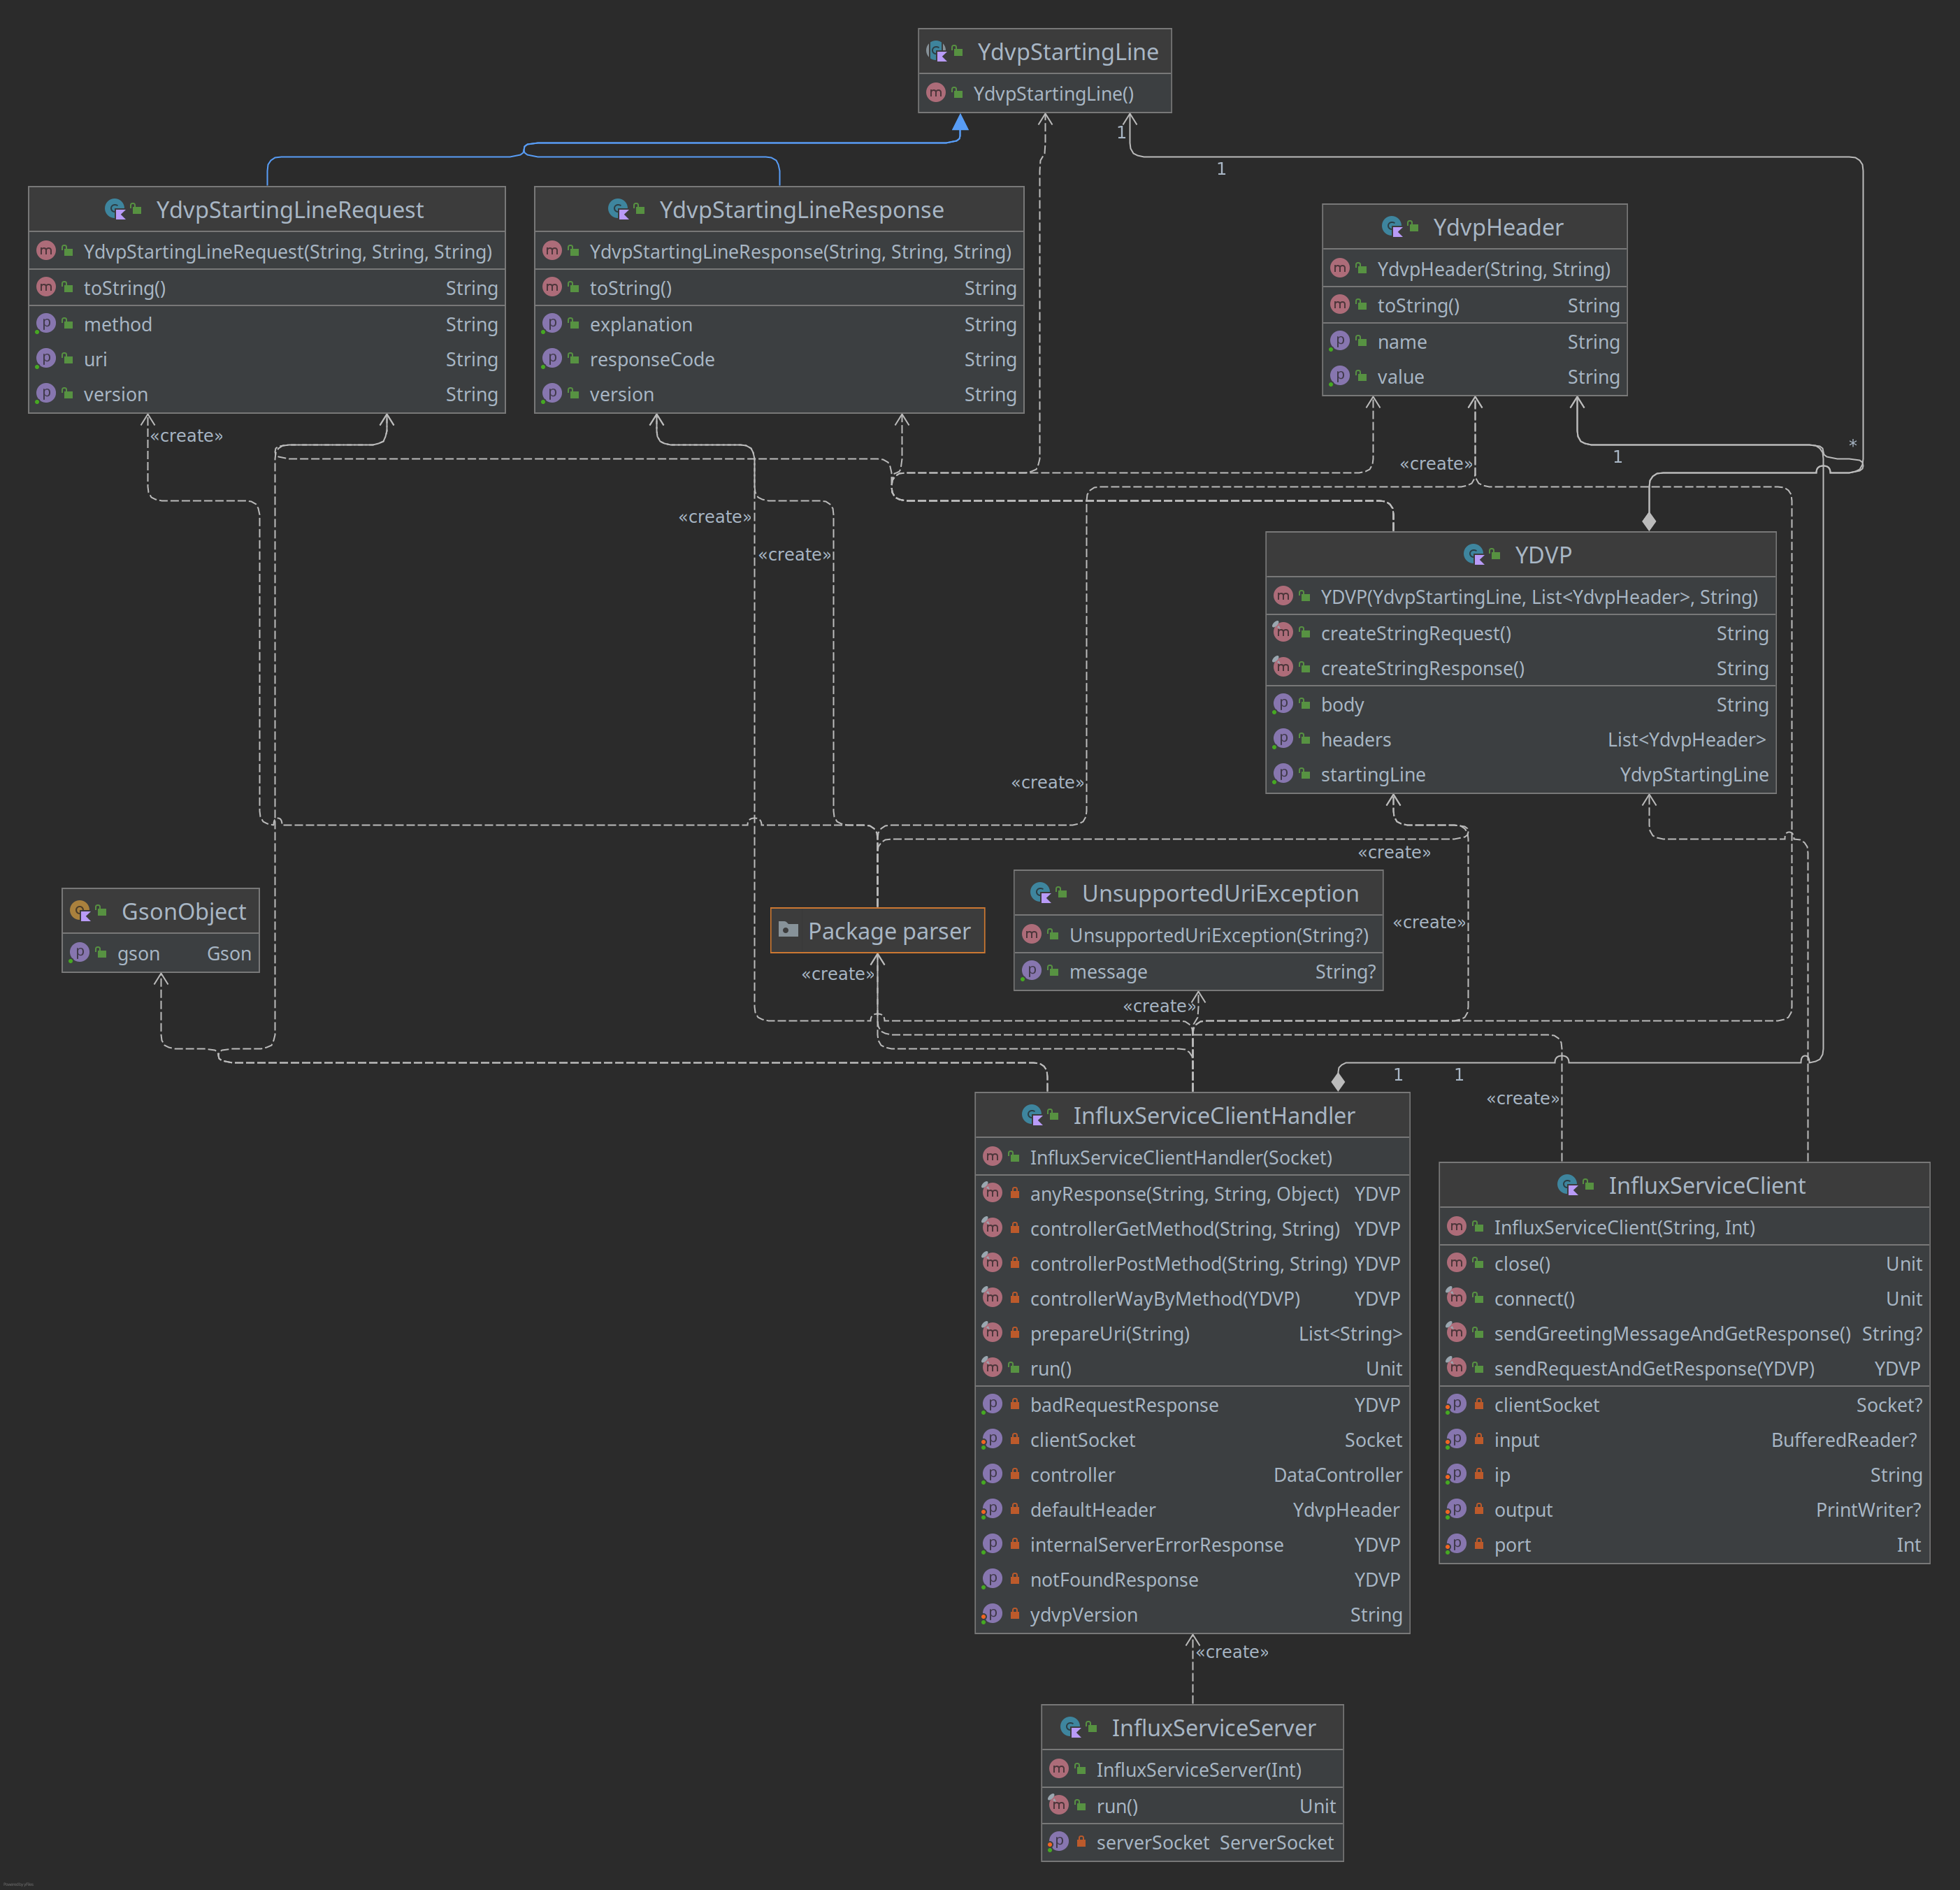
\includegraphics[width=\textwidth]{img/serverDiagram.png}
	\caption{Диаграмма классов серверной части приложения}
	\label{fig:serverAndProtocol}
\end{figure}
\pagebreak

\subsection{Блок-схема работы сервера}
\pagebreak